\chapter{Status quo and solution}
Section dedicated to description of problem and proposition of our application.
\section{Problem description}
\par
A friend of mine reached out to me to ask me in order to ask if I could automate part of his agenda work agenda. Administration of swimming competitions and creating statistics is very repetitive and error-prone list of tasks. However, almost all the tasks are executed in same straightforward order.
\par
The Czech Swimming Federation \footnote{\url{https://www.czechswimming.cz}} structure has to be modeled as objects in the application and database records as a storage. Thus, logical structure should be decided and implemented. Swimming referees belong to clubs, clubs are located in geographical regions. Swimming cup is hosted by club. Each club contains dozen of swimming referees and one of them is a club manager. When a cup is online each referee can sign himself or herself up as available for the cup. Club manager can also sign up members of his club for to attend a cup. At the end of the day, organizer of the cup assigns available referees to positions (dedicated task-related roles during cup) that he finds them suitable for. My friend, the chairman of referee committee should be able to perform additional administration related to the database as whole - such as adding and removing users, creating new clubs and modifying whole structure. Administrator can also notify all visitors by posting news displayed on homepage.
\begin{figure}[h]
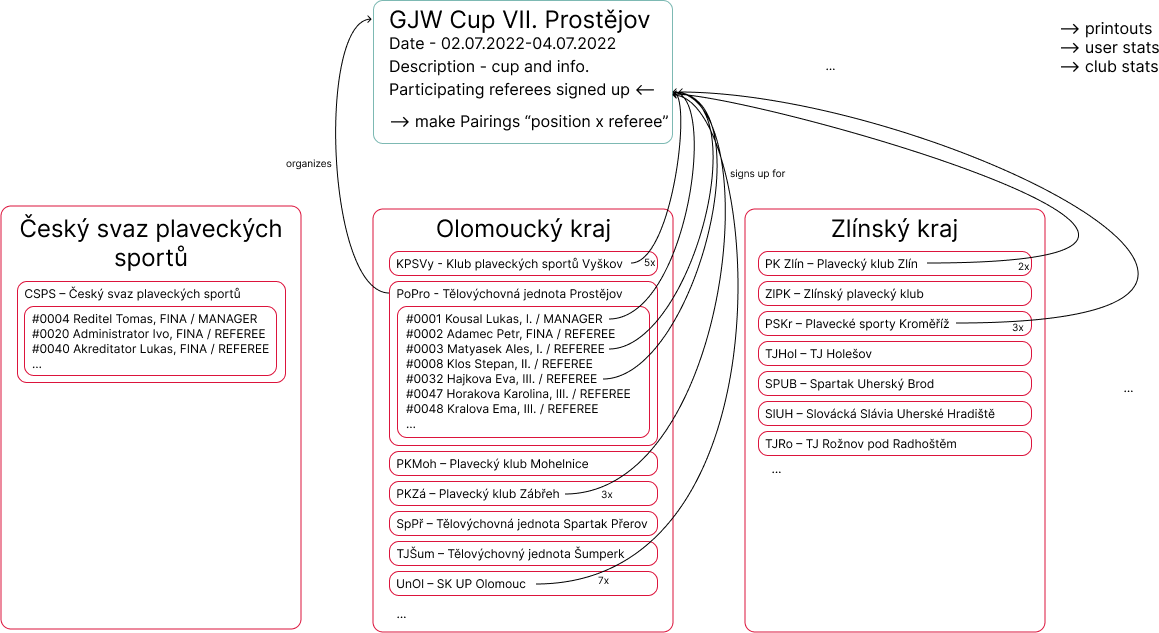
\includegraphics[scale=0.335]{img/swimmpair_schema.png}
\caption{Preview of grouping Regions-Clubs-Users and Cup.}
\label{fig1.1:grouping}
\end{figure}
The SwimmPair system should deliver public listing of all \textbf{users}, \textbf{cups}, \textbf{news}, \textbf{individual statistics} and \textbf{club statistics}. System should allow to browse stats on a yearly basis. Structure from this image then has to be appropriately modeled with objects. Proposition of database schema will be shown further down. 
%\newpage
\section{Stakeholders}
Groups direclty and indirectly interested in existence of this application and breakdown of its active/passive users.
\subsection*{Interest groups}
There are several entities that are interested in existence of this application. All these stakeholders will have their job facilitated and organized better to some extent thanks to this application.  
Interested stakeholders are:
\begin{itemize}
  \item \textbf{Czech Swimming Federation} - organization for swimming,
  \item \textbf{Olomouc Region}, \textbf{Zlin Region} - regions administered together,
  \item \textbf{Lukas K} - manager who demanded this application.
\end{itemize}
\subsection*{Users of application}
Our users are Czech Swimming Federation members. If their \textbf{region} is \textbf{participating in this application}, clubs and referees from this region must be in our system. With regards to referee's competence level within these clubs, one will have one of these roles: 
\begin{itemize}
  \item \textbf{system administrator} ($\sim$1-3),
  \item \textbf{club manager} + also a referee ($\sim$10s),
  \item \textbf{referee} ($\sim$100s).
\end{itemize} 
Roles are self-descriptive and previously casually mentioned. My friend, who came up with this idea is \textbf{system administrator} because he's been running all this agenda offline. Club managers are taking care of competitions on behalf of the club and referees are common people who have some degree of knowledge about competitions. Colected statistics will then be used for accreditation granting, activity monitoring and categorization overall.
\par
We were iterating form and features of the web application with two future system administrators during time of development. We then tested usability on all three groups of users via. SUS \footnote{\textbf{System Usability Scale} is a questionnaire to reveal how friendly tested system is to target audience. We carried on initial testing for 20 people belonging to one of these 3 categories to find out if we met at least an average score which was determined to be 68/100.} questionnaire.
%%%An~example citation: %\cite{Andel07}
\section{Functional requirements}
There are some related bundles of tasks that we would like to solve within our application by implementing features and pages to solved them.
\subsection*{"C" as Cup administration}
\begin{enumerate}
    \item \lbrack club manager\rbrack \,needs to\, \lbrack create swimming cup\rbrack \,in order to\, \lbrack publish cup and invite others to participate\rbrack
    \item \lbrack club manager\rbrack \,needs to\, \lbrack create pairing for swimming cup\rbrack \,in order to\, \lbrack finalize preparations of cup the day before it takes place\rbrack
    \item \lbrack club manager\rbrack \,needs to\, \lbrack preview cups and print pairing\rbrack \,in order to\, \lbrack perform inspection and publish information offline\rbrack
    \item \lbrack club manager\rbrack \,needs to\, \lbrack participate in cup or participate with teammates\rbrack \, in order to\, \lbrack help with swimming cup to happen\rbrack
\end{enumerate} 
\subsection*{"R" as Referees administration \& overview}
\begin{enumerate}
\item \lbrack club manager\rbrack \,needs to\, \lbrack manage swimming club\rbrack \,in order to\, \lbrack keep information and users up-to-date\rbrack
\item \lbrack club manager\rbrack \,needs to\, \lbrack perform referees managment\rbrack \, in order to \, \lbrack keep referees up-to-date\rbrack
\item \lbrack referee\rbrack \,needs to\, \lbrack view statistics of referees\rbrack \, in order to \, \lbrack have track record about participation\rbrack
\item \lbrack club manager\rbrack \,needs to\, \lbrack view statistics of clubs\rbrack \, in order to \, \lbrack have information about performance of own club\rbrack
\item \lbrack club manager\rbrack \,needs to\, \lbrack perform club managment\rbrack \, in order to \, \lbrack keep own club up-to-date\rbrack
\item \lbrack system administrator\rbrack \,needs to\, \lbrack manage referees\rbrack \, in order to \, \lbrack add, remove, update users in the application\rbrack
\item \lbrack system administrator\rbrack \,needs to\, \lbrack list referees overview\rbrack \, in order to \, \lbrack see activity of referees\rbrack
\end{enumerate} 
\subsection*{"S" as Stakeholders interests}
\begin{enumerate}
  \item \lbrack system administrator\rbrack \,needs to\, \lbrack have overview of clubs\rbrack \, in order to \, \lbrack be informed about happenings (within application)\rbrack
  \item \lbrack stakeholder\rbrack \,needs to\, \lbrack have overall categorization of federation\rbrack \, in order to \, \lbrack use system for administrative purposes\rbrack
  \item \lbrack stakeholder\rbrack \,needs to\, \lbrack have database archivation of federation\rbrack \, in order to \, \lbrack use system as archivation tool\rbrack
  \item \lbrack stakeholder\rbrack \,needs to\, \lbrack have information about participations\rbrack \, in order to\, \lbrack grant accreditations to referees\rbrack
  \item \lbrack system administrator\rbrack \,needs to\, \lbrack publish news\rbrack \, in order to \, \lbrack notify everybody about new things\rbrack
  \item \lbrack system administrator\rbrack \,needs to\, \lbrack edit page/s\rbrack \, in order to \, \lbrack change public info page\rbrack
\end{enumerate}
\section{Domain model}
Let's go through entities that have to be represented in our system one by one starting from the most important ones. We will outlay entities and their relations. After that basic idea of entities and their relations will be established we proceed to project specification for further implementation endeavours. We, however, worked more iteratively so this is just retrospective domain model for implementation that we were specifying during the time of development. 
\par
\subsection*{Cup}
\textbf{Cup is the most important entity.} A swimming Cup contains name, description, date and is affiliated to organizing Club.
Cup serves two purposes. \textbf{Firstly}, assigning referees for specific tasks (time tracking, computer support, head of the cup, etc.) has to be \textbf{ready by the time the event takes place}. \textbf{Secondly}, statistics summing up participations of Referees and Clubs have to be calculated for each year over all cups in this time period. We also have to discriminate between upcoming and already past cups. Upcoming cups should be displayed, past cups should reside in the archive to be revisited for statistical purposes.
\iffalse\subsection*{User - strike}
\par
User is an entity modelling swimming referee. A referee participating in this system falls in one of three categories. These categories or levels if you wish are \textbf{referee}, \textbf{club manager} and \textbf{system administrator}. User has to be uniquely identifiable. A person i.e. User in the system is going to have profile information such as first name, family name, email address. Good practice of using email address as a login information is going to be used here. User must also contain SwimmPair hierarchy listed above\footnote{\textbf{Rights} - referee 0 / club manager 1 / system administrator 2} and indicator of one's skill and knowledge in the swimming field, i.e. referee category. User must also belong to exactly one club in our system.
\fi
\subsection*{Referee}
Referee is a person and main workforce during swimming competitions. Referee is a member of Club and participates on it's behalf in Cup. Referee has one of ranks  \footnote{\textbf{Referee Rank} - 1/2/3/4/FINA - \url{https://www.czechswimming.cz/index.php/rozhodci}}. Referee is assigned one or more Position/s, such as \underline{timekeeping} or \underline{pc support} and is charge of. 
\subsection*{Club manager}
Club manager is usually one person who is in charge of administration of Club. Club manager organizes Cup on behalf on Club and acts as main figure during it. Club manager can also help with some work (Position), however, more they are more of an administrative character, if ever. Club manager completes pairing and plans everything. 
\subsection*{Coordinator}
Coordinator is a person who is head of swimming in specific region. He budgets, plans tournaments, manages administrations and whole database of referees, clubs and cups. He's person of highest administrative importance.
\subsection*{Club}
\par
Club is an administrative unit grouping people (in the same city). Club has a specific name, abbrevation and ID in Czech Referee Federation. An image can be included as well. A club will be serving as a formal authority organising Cup by a User who is club manager. Club is unanimously affiliated to Region. Statistics regarding performance of members of Club at swimming competitions must be implemented. Statistics have informative characted and will save time in the current status quo - keeping track of presence and work descriptions in Excel spreadsheets.
\subsection*{Region}
There are 13 regions of the Czech Republic, we are solving this problem for 2 that are being adminstered together. Maybe we will do more. Clubs are located in one of these regions. When new Club starts using SwimmPair in the future, new Region has to be added and potential clubs created and attached to this Region. 

\iffalse
\subsection*{Availability}
Referee is available in the time of Cup.
\fi

\subsection*{Pairing}
Pairing is simple list of pairs (\textbf{Referee} x \textbf{Position}) $\rightarrow$ \textbf{Cup}.
\subsection*{Position}
Predefined list of tasks necessary to be done at each Cup. This list is probably never going to change since there is a fixed set of roles. Referees are going to be assigned to these Positions for each Cup.
\newpage
\subsection*{Schema of entities and connections}
Majority of focus should be on \textbf{Referee}, \textbf{Club manager} and \textbf{Cup} in the presented schema. Referees belong to Club that belong to Region. These two entities \textbf{Referee} and \textbf{Cup} along with \textbf{Position} will then be brought together as \textbf{Pairing} which contains referees that are available for specific cups and will be performing work at specifies position. Referees must be available in specific time but \textbf{Pairing} is where each record can be assigned a position from prescripted \textbf{Positions}.
\begin{figure}[h]
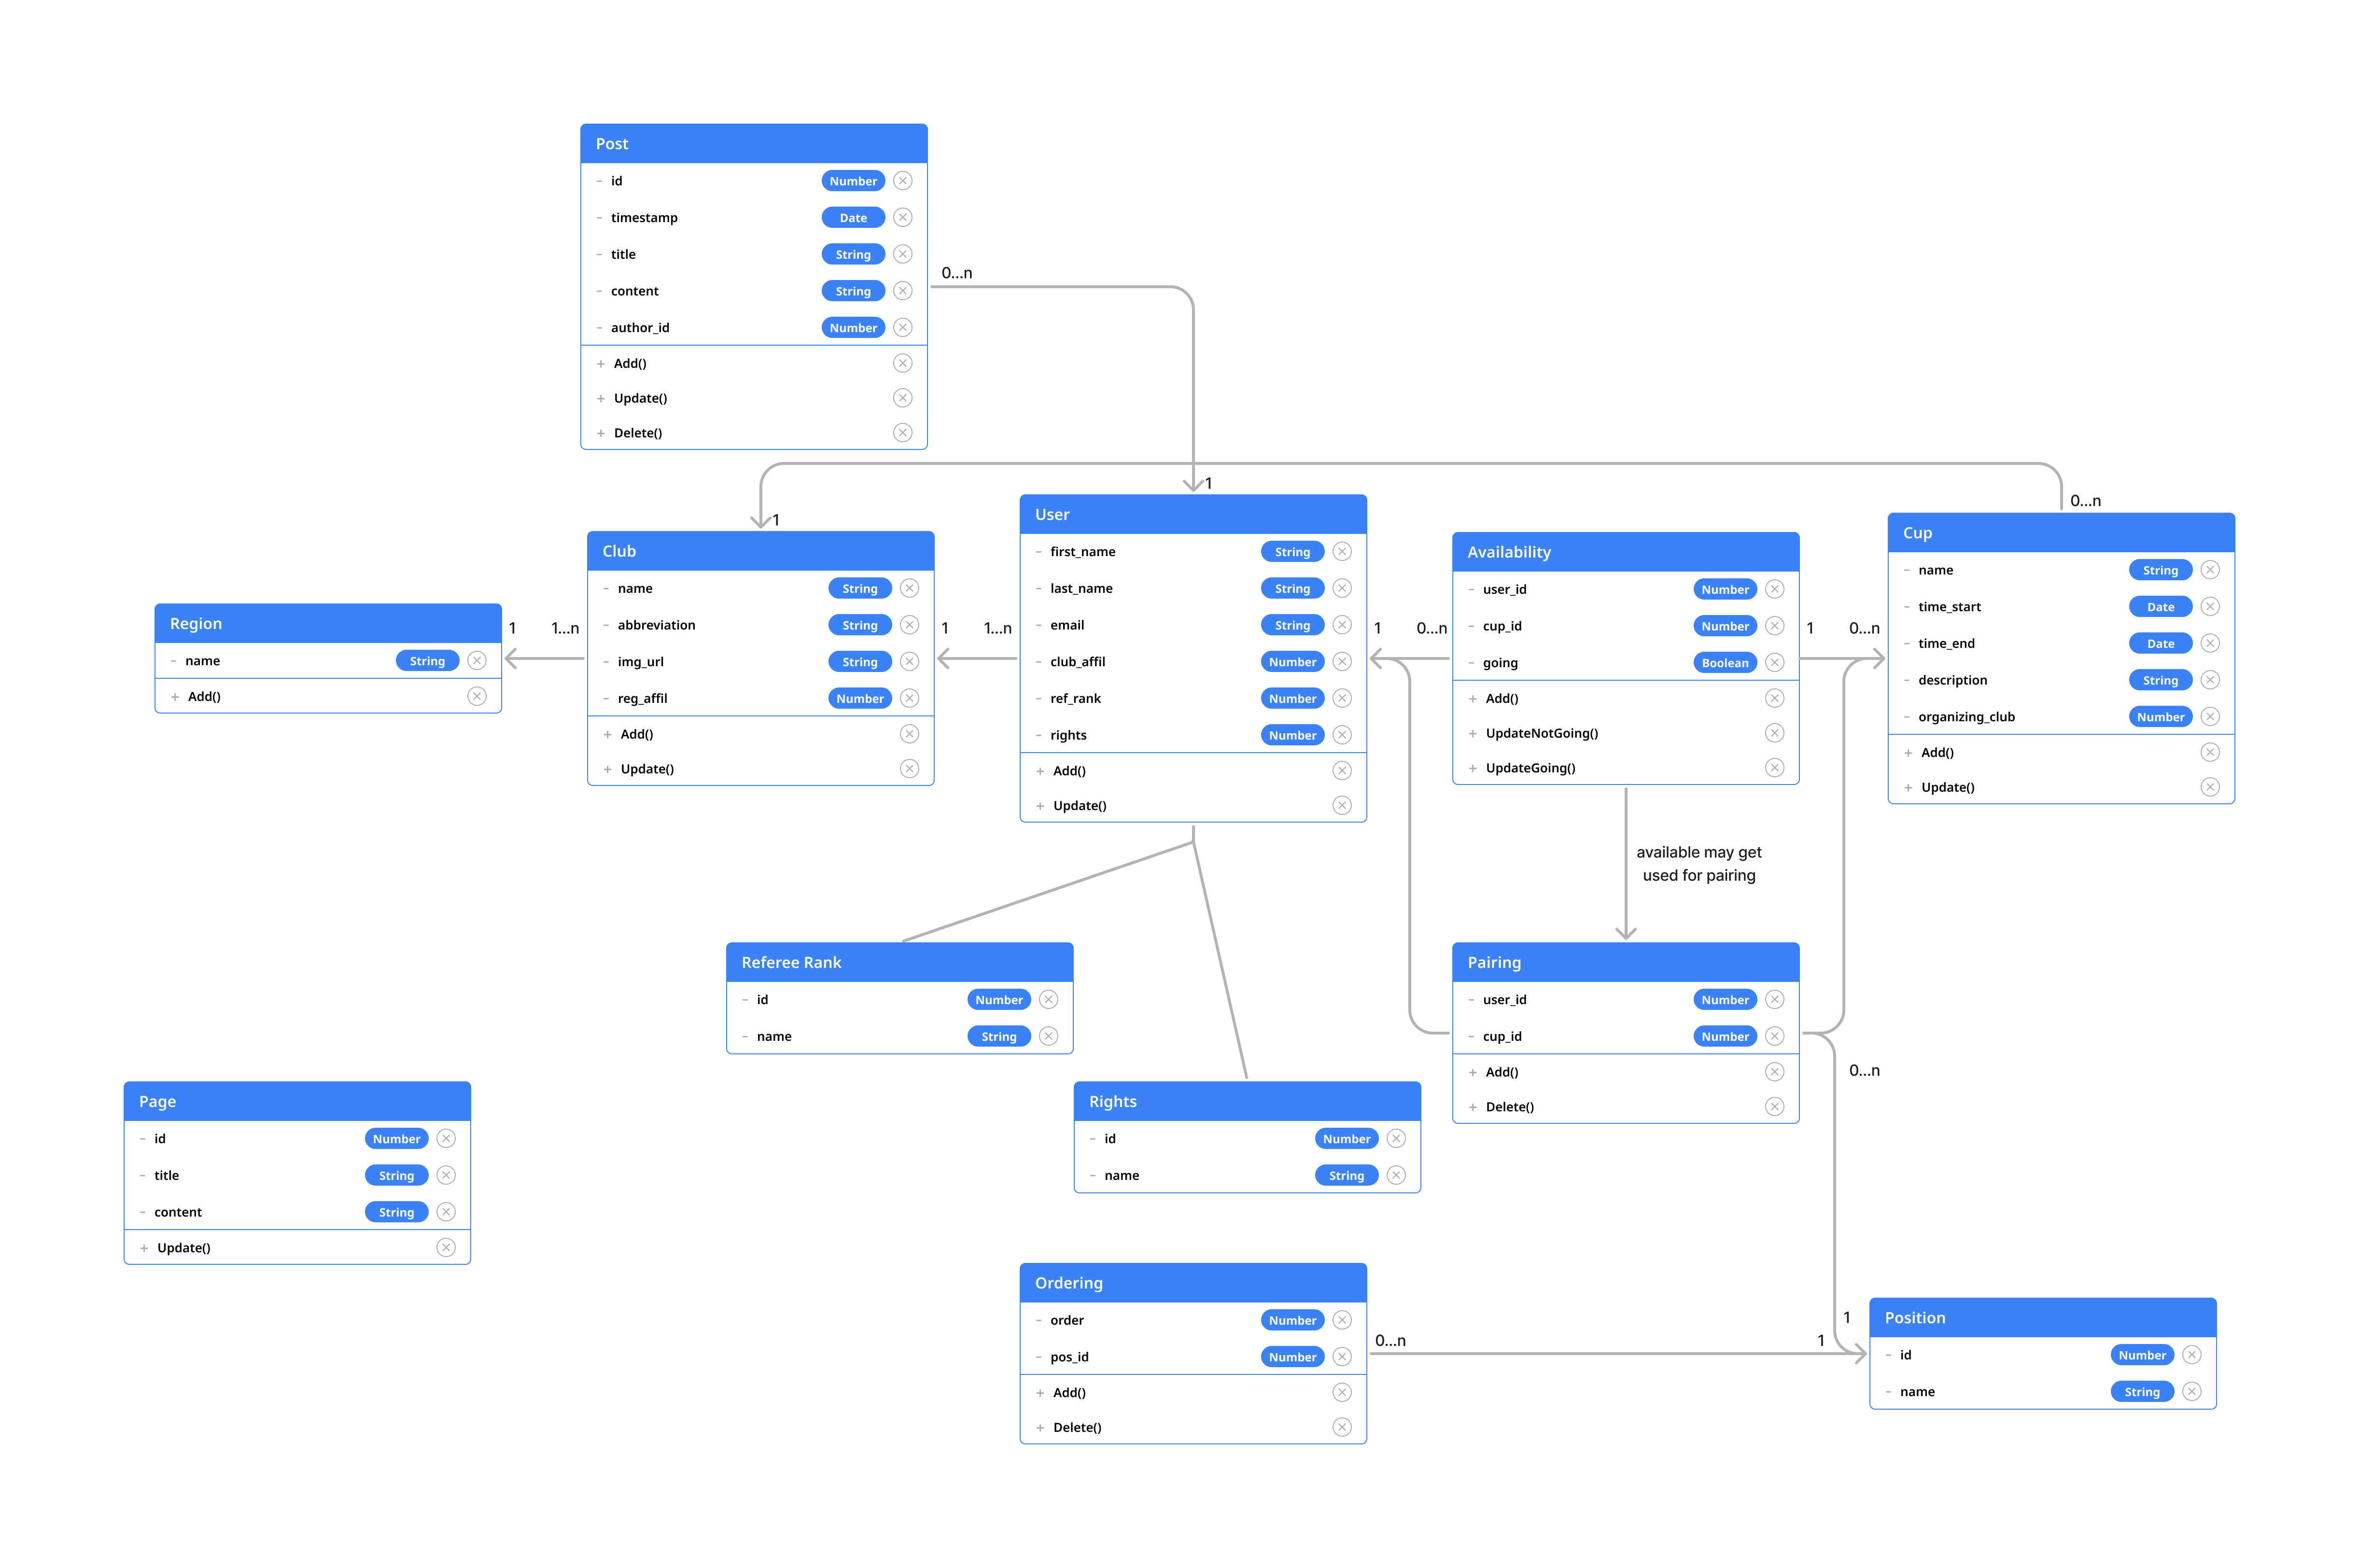
\includegraphics[scale=0.160]{img/swimmpair_uml.png}
  \caption{UML Class Diagram outlaying the situation}
  \label{fig1.2:uml}
\end{figure}
\newpage
\section{Quality/Usability Requirements}
Several good practices have to be implemented to make SwimmPair easy to use. These practices are either well known or situation specific but they have one thing in common - they should make the application good to use.
\subsection*{Smooth frontend browsing}
\par
Frontend of SwimmPair should be easy to use. There are several options and use cases of JavaScript that can come in handy. Reduction of page reloads is definitely a good way to go. Therefore there are going to be asynchronous JavaScript calls for obtain semi-partial data. After, next function will modify the DOM based on data received from asynchronous call. 
\subsection*{Multiple device types}
\par
Today is certain that there are users who want to browse our system from pc, tablet or smartphone and responsive design is a necessity. Since CSS3 supports media queries\footnote{\url{https://developer.mozilla.org/en-US/docs/Web/CSS/Media_Queries}} we are going to use them for creation of device specific styling.
\subsection*{Assigning referees to positions via. drag'n'drop}
\par
Assigning referees to positions for cups should be implemented via drag'n'drop. Dragging a referee, moving referee over the region specified for the positions and releasing mouse button. Double clicking this person is a good way of removing it.
\subsection*{Printouts of pairing}
Upcoming Cup can be directly printed\footnote{\url{https://developer.mozilla.org/en-US/docs/Web/CSS/Media_Queries/Using_media_queries\#targeting_media_types}} from website and hanged as data printout. 
%\subsection*{Mobile administration}
%Since some things could be done from phone, a phone app without a necessity of web browser will have more native feel. Assigning by drag and drop would be very %hazardeous to do with regards to difference between mouse and finger. Also we are not certain that the Events are the same. Therefore full version %adminsitrative app should be necessary to be provided.
\subsection*{Appropriate design}
\par
Red blue and grey are colors that appear pretty much at a swimming pools. These colors will be used in our system as well. The elements should have fresh lightweave look and not appear heavy.
